\ifx\mainfile\undefined
%  ========================================================================
%  Copyright (c) 2006-2011 The University of Washington
%
%  Licensed under the Apache License, Version 2.0 (the "License");
%  you may not use this file except in compliance with the License.
%  You may obtain a copy of the License at
%
%      http://www.apache.org/licenses/LICENSE-2.0
%
%  Unless required by applicable law or agreed to in writing, software
%  distributed under the License is distributed on an "AS IS" BASIS,
%  WITHOUT WARRANTIES OR CONDITIONS OF ANY KIND, either express or implied.
%  See the License for the specific language governing permissions and
%  limitations under the License.
%  ========================================================================
%
 
\documentclass [11pt, twoside] {uwthesis}

\usepackage{color}
\usepackage{url}
\usepackage{amsmath}
\usepackage{amsfonts}
\usepackage[bookmarks,
	hidelinks,
	plainpages=false,
	pdfpagelabels,
	pagebackref=true,
            ]{hyperref}
\renewcommand*{\backref}[1]{}% for backref < 1.33 necessary
\renewcommand*{\backrefalt}[4]{%
  \ifcase #1 %
    (No citations.)%
  \or
    (Cited on page #2.)%
  \else
    (Cited on pages #2.)%
  \fi
}

\newcommand{\biburl}[1]{{\tt<}\url{#1}{\tt>}}

\hypersetup{%
pdfauthor = {Daniel Chaim Halperin},
pdftitle = {Simplifying the Configuration of 802.11 Wireless Networks with Effective SNR},
pdfsubject = {Ph.D. Dissertation},
pdfkeywords = {},
pdfcreator = {University of Washington, Computer Science and Engineering},
pdfproducer = {},
bookmarksopen = {true},
pdfpagelayout = {TwoColumnRight},
}

\usepackage{footnotebackref}
%%%%%%%%%%%%%%%%%%%%%%%%%%%%%%%%%%%%%%%%%%%%%%%%%%%%%%
%%%        Formatting sections                     %%%
%%%%%%%%%%%%%%%%%%%%%%%%%%%%%%%%%%%%%%%%%%%%%%%%%%%%%%
\newcommand{\algref}[1]{Algorithm~\ref{#1}}
\newcommand{\chapref}[1]{Chapter~\ref{#1}}
\renewcommand{\eqref}[1]{Equation~\ref{#1}}
\newcommand{\figref}[1]{Figure~\ref{#1}}
\newcommand{\secref}[1]{\S\ref{#1}}
\newcommand{\tabref}[1]{Table~\ref{#1}}
\newcommand{\heading}[1]{\vspace{4pt}\noindent\textbf{#1}}
\newcommand{\topheading}[1]{\noindent\textbf{#1}}
\newcommand{\noheading}[0]{\vspace{4pt}\noindent}

%%%%%%%%%%%%%%%%%%%%%%%%%%%%%%%%%%%%%%%%%%%%%%%%%%%%%%
%%%        XXX and other warnings                  %%%
%%%%%%%%%%%%%%%%%%%%%%%%%%%%%%%%%%%%%%%%%%%%%%%%%%%%%%
\newcommand{\xxx}[1]{\textit{\color{red}XXX #1}}

%%%%%%%%%%%%%%%%%%%%%%%%%%%%%%%%%%%%%%%%%%%%%%%%%%%%%%
%%%        Units                                   %%%
%%%%%%%%%%%%%%%%%%%%%%%%%%%%%%%%%%%%%%%%%%%%%%%%%%%%%%
\usepackage{xspace}
\newcommand{\unitsep}{\texorpdfstring{\,}{ }}
\def\unit#1{% from: http://www.tex.ac.uk/cgi-bin/texfaq2html?label=csname "Defining a macro from an argument"
  \expandafter\def\csname #1\endcsname{\unitsep\text{#1}\xspace}%
}
\def\varunit#1#2{% from: http://www.tex.ac.uk/cgi-bin/texfaq2html?label=csname "Defining a macro from an argument"
  \expandafter\def\csname #1\endcsname{\unitsep\text{#2}\xspace}%
}
\unit{GHz}
\unit{MHz}
\unit{kHz}
\unit{Gbps}
\unit{Mbps}
\unit{KB}
\unit{dB}
\unit{dBi}
\unit{dBm}
\unit{W}
\unit{mW}
\varunit{uW}{$\mu$W}
\unit{ms}
\varunit{us}{$\mu$s}
\unit{h}
\unit{m}
\unit{s}
\unit{km}
\unit{cm}
\unit{mm}
\varunit{mmsq}{mm$^\text{2}$}
\varunit{insq}{in$^\text{2}$}
\newcommand{\degree}{\ensuremath{^\circ}\xspace}
\newcommand{\degrees}{\degree}
%%%%%%%%%%%%%%%%%%%%%%%%%%%%%%%%%%%%%%%%%%%%%%%%%%%%%%%%%%%%%%%%%%%%%%%%%%%%%%%%%%%%%%
% Euler for math | Palatino for rm | Helvetica for ss | Courier for tt
%
% From: http://www.tug.org/mactex/fonts/LaTeX_Preamble-Font_Choices.html
%%%%%%%%%%%%%%%%%%%%%%%%%%%%%%%%%%%%%%%%%%%%%%%%%%%%%%%%%%%%%%%%%%%%%%%%%%%%%%%%%%%%%%
\renewcommand{\rmdefault}{ppl} % rm
\usepackage[scaled]{helvet} % ss
\usepackage{courier} % tt
\usepackage{eulervm} % a better implementation of the euler package (not in gwTeX)
\normalfont
\usepackage[T1]{fontenc}
%%%%%%%%%%%%%%%%%%%%%%%%%%%%%%%%%%%%%%%%%%%%%%%%%%%%%%%%%%%%%%%%%%%%%%%%%%%%%%%%%%%%%%

%%%%%%%%%%%%%%%%%%%%%%%%%%%%%%%%%%%%%%%%%%%%%%%%%%%%%%
%%%        Figures                                 %%%
%%%%%%%%%%%%%%%%%%%%%%%%%%%%%%%%%%%%%%%%%%%%%%%%%%%%%%
\usepackage{graphicx}
% Caption package both lets you set the spacing between figure and caption
% and also makes the \figref{} point to the right place.
\usepackage[font=bf,aboveskip=6pt,belowskip=-4mm]{caption}
% Allow subfigures, make them bold
\usepackage[bf,BF,small]{subfigure}
% List of figures
\setcounter{lofdepth}{2}  % Print the chapter and sections to the lot

%%%%%%%%%%%%%%%%%%%%%%%%%%%%%%%%%%%%%%%%%%%%%%%%%%%%%%
%%%        Lists with reduced spacing              %%%
%%%%%%%%%%%%%%%%%%%%%%%%%%%%%%%%%%%%%%%%%%%%%%%%%%%%%%
\usepackage{enumitem}

%%%%%%%%%%%%%%%%%%%%%%%%%%%%%%%%%%%%%%%%%%%%%%%%%%%%%%
%%%        Fancy tables                            %%%
%%%%%%%%%%%%%%%%%%%%%%%%%%%%%%%%%%%%%%%%%%%%%%%%%%%%%%
\usepackage{tabulary}
\usepackage{booktabs}

%%%%%%%%%%%%%%%%%%%%%%%%%%%%%%%%%%%%%%%%%%%%%%%%%%%%%%
%%%        Formatting techniques/tools/etc.        %%%
%%%%%%%%%%%%%%%%%%%%%%%%%%%%%%%%%%%%%%%%%%%%%%%%%%%%%%
\newcommand{\term}[1]{\texttt{#1}}

\begin{document}
 
\textpages
\setcounter{chapter}{5} % Set to n-1!
\fi
%%%%%%%%%%%%%%%%%%%%%%%%%%%%%%%%%%

\cleardoublepage
\chapter{Packet Delivery over MIMO Channels}
\label{chap:delivery}

In this section, we use our testbeds to experimentally evaluate how well our Effective SNR model predicts packet delivery. This is the fundamental measure of whether the model is useful; good predictions enable applications such as rate adaptation, transmit power control, antenna selection, and channel selection.

\begin{figure*}[ht]
	\centering
	\subfigure[Single spatial stream, single receive antenna (1x1)]{
		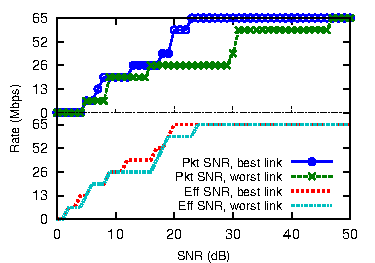
\includegraphics[width=0.49\textwidth, clip]{figures/esnr/embed_ratestep_snr_1x1_90.pdf}%
		\label{fig:snr_rate_step_1x1}%
	}\hfill%
	\subfigure[Single spatial stream, three receive antennas (1x3)]{
		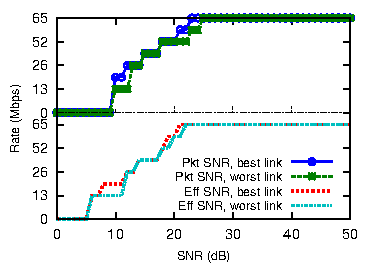
\includegraphics[width=0.49\textwidth, clip]{figures/esnr/embed_ratestep_snr_1x3_90.pdf}%
		\label{fig:snr_rate_step_1x3}%
	}
	
	\subfigure[Two spatial streams, three receive antennas (2x3)]{
		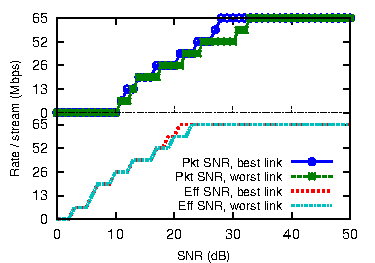
\includegraphics[width=0.49\textwidth, clip]{figures/esnr/embed_ratestep_snr_2x3_90.pdf}%
		\label{fig:snr_rate_step_2x3}%
	}\hfill%
	\subfigure[Three spatial streams, three receive antennas (3x3)]{
		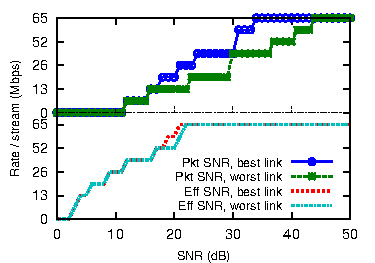
\includegraphics[width=0.49\textwidth, clip]{figures/esnr/embed_ratestep_snr_3x3_90.pdf}%
		\label{fig:snr_rate_step_3x3}%
	}
	\caption{\label{fig:snr_rate_steps}The variation of best rate with SNR over links and antenna configurations. Excepting extremely low and high SNRs, one RSSI-based packet SNR value maps to multiple best rates for different links, %. For the same data, 
while Effective SNR provides a clear indicator of the best rate for nearly all links.}
\end{figure*}

\heading{Measurement setup.}
We first measure packet delivery for different antenna configurations over a 20\MHz channel on two \program{iwl5300} testbeds, one at UW CSE and one at Intel Labs Seattle. The 1x1 or SISO configuration corresponds to 802.11a, where each node has a single transmit or receive antenna. In addition we measure configurations with three receive antennas and 1, 2, or 3 spatial streams. These 1x3, 2x3 and 3x3 MIMO configurations are only available with 802.11n. They exploit \emph{spatial diversity} and \emph{spatial multiplexing} to greatly increase performance.

In each test, we send 1500 byte packets as constant bit-rate UDP traffic generated by \program{iperf} at 2\Mbps for 5 seconds. 
We turn off link layer retransmissions to observe the underlying packet delivery rate, and fix the link data rate and the transmit power in each run. Then we collect packet reception rate (PRR) statistics for all 8 rates using 1, 2, and 3 spatial streams as we vary the power between $-$10\dBm and $+$16\dBm in steps of 2\dB.

The receiver also records the CSI and per antenna RSSIs to measure the RF channel for each correctly received packet. Note that CSI is measured during the preamble, so it does not depend on the transmit rate. Similarly, 3x3 CSI gives us the channel between each pair of transmit and receive antennas, so it also implicitly contains 1x1 CSI\@. To get a single SNR value with multiple receive antennas, we first convert the per-antenna RSSIs to SNRs and then sum the SNRs.
This is a straightforward choice for a single spatial stream as it corresponds to receiver processing using MRC~\cite{Goldsmith}.
It is also reasonable for 2- and 3-stream MIMO because the streams are interleaved.

The above testing gives us ground truth data to probe variation across 200 links, 26\dB of transmit power, four antenna configurations ranging from 1x1 to 3x3, and 8 per stream rates (for 24 rates with up to three streams). This covers all of the key variables in our delivery model.

\heading{Result: Rate Confusion.} To understand whether the Effective SNR model accurately predicts packet delivery, we analyze our measurements for the highest supported rate (PRR$\geq$ 90\%) for each link and all NIC settings. The results are shown in \figref{fig:snr_rate_steps}, broken down by antenna configuration. \figref{fig:snr_rate_step_1x1} shows 1x1 rates for both testbeds combined. \figref{fig:snr_rate_step_1x3}--\ref{fig:snr_rate_step_3x3}  show rates for 1x3, 2x3 and 3x3 configurations for the Intel testbed; it is denser than UW and supports MIMO experiments over our NIC's transmit power range.
For each RSSI-based SNR or Effective SNR value, we find the best link (with the fastest best rate) and the worst link (with the slowest best rate). We plot the spread of their fastest rates in these graphs.\footnote{\figref{fig:snr_rate_step_1x3} does not include data for 1x3 at 6.5\Mbps, because very few links experience loss at that rate.}

Ideally, the best and worst lines would overlap completely. %and form a single staircase. 
That is, the highest rate for a given SNR would be the same for the best and worst links. This rate would then be an accurate prediction for the Effective SNR or packet SNR level. Conversely, gaps between the best and worst lines expose confusion about which rate will be the highest rate for that SNR\@.

In the top two lines of the 1x1 and 3x3 cases, we see that the RSSI-based SNR does have a large spread between the best and worst lines. Except for extremely low and high SNRs, nearly all SNRs have at least two and up to five different rates as suitable choices for the best rate. That is, RSSI often poorly indicates rate.

In sharp contrast, %looking at bottom lines in the graphs, 
the two Effective SNR lines overlap almost all the time, and mostly appear to be a single line. This is almost an ideal result. Effective SNR is a clear indicator of best rate. When there is slight separation, the spread is only between rates that use the same modulation but different amounts of coding. These combinations are also close together in our wired experiments. 

Interestingly, we see that RSSI-based predictions are much better for the 1x3 and 2x3 cases, though still not as accurate as Effective SNR, particularly for the high rates. The reason is \emph{spatial diversity}: spare receive antennas gather the received signal and combine to make the channel more frequency-flat. The effect is well-known, though typically not observable using real 802.11 NICs. It suggests that RSSI is a reasonable predictor for an 802.11 configuration with significant diversity. However, observe that RSSI does not transfer well across the antenna modes (as diversity gains and inter-stream interference change unpredictably) which makes this less useful. This is one reason that SISO rate adaptation schemes do not translate to MIMO\@.

We conclude that Effective SNR consistently and accurately indicates the best rate for nearly all links and all configurations without any per-link calibration. From now on, we use the thresholds in these graphs to predict the working rate for any link. They agree with the measured SNRs on a wired link (\figref{fig:snr_prr_attenuator}), which strongly suggests that the Effective SNR captures the fundamental error characteristics of the link. 

Finally, we note that neither Effective SNR nor RSSI performs well at the lowest modulation at low SNRs. We believe this artifact arises from errors in the AGC values reported by the NIC, observed by Judd et al.~\cite{Judd_CHARM} and confirmed by our data for Intel's hardware.

\heading{Further results.} This results are a subset of those presented in~\cite{Halperin_ESNR}. Though we do not reproduce them all here, the full paper shows that links viewed through the Effective SNR lens have a narrow transition region, much closer to the wired link model of \figref{fig:snr_prr_attenuator} than the wireless links and packet SNR as in \figref{fig:rssi_predictions}. We also demonstrate that the Effective SNR model enables a sender to accurately prune excess transmit power from a strong link while maintaining high packet delivery.

%%%%%%%%%%%%%%%%%%%%%%%%%%%%%%%%%%
\ifx\mainfile\undefined
%
% ==========   Bibliography   ==========
%
%\nocite{*}   % include everything in the uwthesis.bib file
\bibliographystyle{plain}
\bibliography{dhalperi_thesis}

\end{document}
\fi
